\scanpage{26}
\deleted{
\deleted{Comme $T_p(u)$ et $T_p(u^*)$ sont}

En effet, d'après la théorie $p$-adique \inserted{de Serre} (ou th. cohomologique de Weil, on aura
\[
(*)\quad \deg u=\det T_p(u)_{\mathrm{ét}}\det T_p(u^*)_{\mathrm{ét}},
\]
\margin{$\unsure{-\,=}$}
et il reste à prouver que
\[
1^\circ)\quad T_p(u)_{\mathrm{ét}}=T_p(u^*)_{\mathrm{ét}}
\]
\margin{\figure{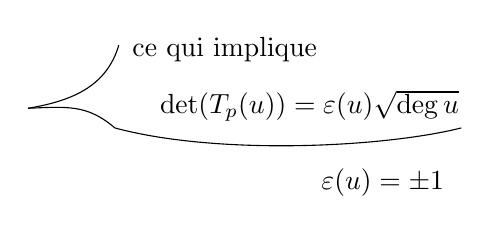
\begin{tikzpicture}[x=1cm,y=1cm]
\draw (0,0) .. controls (.6,.1) and (1,.3) .. (1.15,.8);
\draw (0,0) .. controls (.5,.02) and (.75,.05) .. (1.1,-.25) .. controls (2.4,-.6) and (4.5,-.5) .. (5.5,-.25);
\node[anchor=west] at (1.2,.75) {ce qui implique};
\node[anchor=west] at (1.55,.03) {$\det(T_p(u))=\varepsilon(u)\sqrt{\deg u}$};
\node[anchor=west] at (3.6,-.95) {$\varepsilon(u)=\pm1$};
\end{tikzpicture}}}
\[
2^\circ)\quad\varepsilon(u)=1
\]
D'ailleurs on peut \inserted{se borner à} supposer $u\in\operatorname{Hom}(A,A)\otimes_{\mathbb Z}\mathbb Q\underset{\unsure{\varepsilon}}{=}E$, et alors $\varepsilon$ est un hom
\[
E^*\longrightarrow(+1,-1),\quad\deleted{\unsure{de gr.}}
\]
qui est une fonction rationnelle (quotient de deux fonctions
\deleted{\unsure{on sait} \unsure{que tout tel hom.} \unsure{est égal}}
}

\mspage{25}
